\chapter{Decision Trees}
\label{ch:decision-trees}

\chapterguide%
  {\chapref{ch:training} plus basic probability from \chapref{ch:statistics}; entropy is helpful but re-explained here.}
  {Grow a classification tree by hand using Gini impurity and information gain, build regression trees with variance reduction, and control tree size with stopping rules and pruning.}

A decision tree predicts by asking a sequence of simple questions --- ``is age below 30?'', ``is income at least 50{,}000?'' --- and routing each observation down the branches until it reaches a \term{leaf}, which holds the prediction. Small trees are among the most human-readable models: their learned rules can be printed, drawn, and discussed. Trees are also the building blocks of random forests and gradient boosting (\chapref{ch:ensembles}), two strong families for tabular data.

\begin{firstread}
A decision tree is a flowchart learned from examples. Training chooses questions that separate the known answers well. Prediction follows one path of yes/no answers to a final box. \term{Impurity} is only a score for how mixed the answers remain in a box.
\end{firstread}

\begin{mlfigure}
\begin{tikzpicture}[
  font=\small,
  qnode/.style={draw, rounded corners=2pt, align=center, fill=gray!10, inner sep=4pt},
  leaf/.style={draw, align=center, inner sep=4pt},
  level distance=1.35cm,
  level 1/.style={sibling distance=4.6cm},
  level 2/.style={sibling distance=2.4cm},
  edge from parent/.style={draw, -{Stealth[length=1.8mm]}}
]
\node[qnode] {age $<30$?}
  child {node[qnode] {income $\geq 50$k?}
    child {node[leaf] {predict:\\approve}
      edge from parent node[left=1pt] {yes}}
    child {node[leaf] {predict:\\review}
      edge from parent node[right=1pt] {no}}
    edge from parent node[left=2pt] {yes}}
  child {node[leaf] {predict:\\approve}
    edge from parent node[right=2pt] {no}};
\end{tikzpicture}
\end{mlfigure}

\begin{intuition}
A decision tree is a flowchart of yes/no questions, like the game ``twenty questions.'' Training is simply the process of discovering which question to ask first, second, and third so that each question splits the data as cleanly as possible.
\end{intuition}

\section{How a tree is grown}
\label{sec:decision-tree}

Standard tree learning (the CART algorithm) is \term{greedy and recursive}:

\begin{enumerate}
  \item At the current node, consider candidate splits: for a numerical feature, thresholds between sorted values; for categorical features, the available split rules depend on the tree formulation and representation.
  \item Score each candidate by how much it \emph{purifies} the data --- how well it separates the classes (or, for regression, how much it shrinks the spread of the target).
  \item Apply the best split, sending observations left and right.
  \item Repeat on each child until a stopping rule fires; each final node becomes a leaf that predicts its majority class (classification) or mean target (regression).
\end{enumerate}

Greedy means the algorithm never looks ahead or reconsiders: it takes the best immediate split at every step. That keeps training fast and usually works well, though it does not guarantee the globally best tree.

\section{Measuring impurity}

To pick a split, the algorithm needs a number for ``how mixed is this node?'' With $p_k$ the fraction of class $k$ in a node, two standard measures are the \term{Gini impurity} and the \term{entropy}:
\[
  G=1-\sum_{k=1}^{K}p_k^2,
  \qquad
  H=-\sum_{k=1}^{K}p_k\log_2 p_k.
\]
Both are zero for a pure node (one class only) and largest for a perfect mixture. Gini reads as ``the probability of mislabeling a random point if labels were assigned according to the node's class mix''; entropy reads as ``how many yes/no questions of uncertainty remain.'' A split is chosen to maximize the \term{information gain}: the parent's impurity minus the size-weighted impurity of the children,
\[
  \operatorname{Gain}
  =I(\text{parent})
  -\frac{n_{\mathrm{left}}}{n}I(\text{left})
  -\frac{n_{\mathrm{right}}}{n}I(\text{right}),
\]
where $I$ is either measure. Gini and entropy almost always agree on the best split; Gini is slightly cheaper to compute and is the common default.

\begin{workedexample}
A node holds 10 loan applications: 6 approved ($+$) and 4 rejected ($-$). Its Gini impurity is
$G_{\text{parent}}=1-(0.6^2+0.4^2)=0.48$.

\emph{Candidate split A} produces children $[4+,0-]$ and $[2+,4-]$:
\[
  G_{\text{left}}=0,
  \qquad
  G_{\text{right}}=1-\left[{\left(\tfrac{1}{3}\right)}^2+{\left(\tfrac{2}{3}\right)}^2\right]=\tfrac{4}{9}\approx 0.444,
\]
\[
  \operatorname{Gain}_A
  =0.48-\left(\tfrac{4}{10}\times 0+\tfrac{6}{10}\times 0.444\right)
  =0.48-0.267=0.213.
\]

\emph{Candidate split B} produces children $[3+,2-]$ and $[3+,2-]$. Each child has the same $60/40$ mix as the parent, so each has $G=0.48$, the weighted impurity is unchanged, and $\operatorname{Gain}_B=0$: split B tells us nothing, and split A wins. (Entropy agrees: split A's gain is $0.971-0.551\approx 0.42$ bits.)
\end{workedexample}

\section{Finding the best split}

The split search follows the verbal rule from earlier in the chapter: examine candidate features and thresholds, compute the weighted impurity after each split, and keep the candidate with the largest impurity reduction.

Consider six one-dimensional observations where the classes separate cleanly. If one threshold places every class-$0$ point on one side and every class-$1$ point on the other, both children have zero impurity. The information gain is therefore equal to the parent impurity, which is the largest possible gain for that node.

\begin{libnote}
Different tree formulations may report an observed boundary value or the midpoint between two adjacent observed values. If both thresholds send all training observations to the same children, the fitted partition is identical even though the printed threshold differs. Midpoint thresholds are often convenient because they define a boundary between observations rather than directly on one observation.
\end{libnote}

\section{The geometry: rectangles in feature space}

Because every question compares one feature to one threshold, a tree carves feature space into axis-aligned rectangles, one per leaf, and predicts a constant inside each.

\begin{mlfigure}
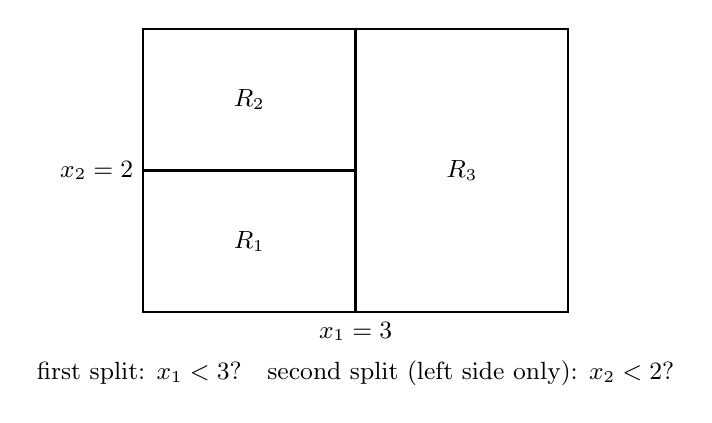
\begin{tikzpicture}[scale=0.9, font=\small]
\draw[thick] (0,0) rectangle (6,4);
\draw[thick] (3,0) -- (3,4);
\draw[thick] (0,2) -- (3,2);
\node at (1.5,1) {$R_1$};
\node at (1.5,3) {$R_2$};
\node at (4.5,2) {$R_3$};
\node[below] at (3,0) {$x_1=3$};
\node[left] at (0,2) {$x_2=2$};
\node[below] at (3,-0.55) {first split: $x_1<3$?\quad second split (left side only): $x_2<2$?};
\end{tikzpicture}
\end{mlfigure}

This geometry explains both a strength and a weakness: boundaries that align with the axes (rules, thresholds, interactions of a few features) are captured perfectly, while a simple diagonal boundary must be approximated by a staircase of many small splits.

\section{Regression trees}

For a numerical target, impurity becomes the spread of $y$ within a node --- its variance (equivalently, the mean squared error around the node mean) --- and a split is chosen to reduce it the most. Each leaf predicts the mean target of its training observations, so the fitted function is piecewise constant.

\begin{workedexample}
A node holds targets $y=\{2,3,10,11\}$ with mean $6.5$ and variance $16.25$. Splitting into $\{2,3\}$ and $\{10,11\}$ gives children with means $2.5$ and $10.5$ and variance $0.25$ each --- a weighted variance of $0.25$. The split explains almost all the spread, and the two leaves predict $2.5$ and $10.5$.
\end{workedexample}

One consequence deserves a warning label: a regression tree can never predict a value outside the range of its training targets. Asked about a house larger than any it has seen, it predicts the mean of its largest-house leaf --- trees do not extrapolate.

\section{Stopping and pruning}

An unrestricted tree keeps splitting until every leaf is pure --- typically one training observation per leaf, which is memorization, not learning. Two complementary defenses:

\begin{mltable}
\renewcommand{\arraystretch}{1.16}
\setlength{\tabcolsep}{5pt}
\begin{tabularx}{\linewidth}{@{}>{\footnotesize\bfseries\leavevmode\color{MLNavy}}p{0.22\linewidth}>{\footnotesize}p{0.40\linewidth}>{\footnotesize}X@{}}
\toprule
\rowcolor{MLPaleBlue!92}
\normalfont\bfseries Method & \bfseries How it works & \bfseries Trade-off \\
\midrule
Pre-pruning (early stopping) & Refuse to grow past limits set in advance: a maximum depth, a minimum number of observations required to split a node or to sit in a leaf, or a minimum impurity decrease. & Simple and fast; the limits are hyperparameters tuned on validation data. \\
Post-pruning & Grow a deliberately large tree first, then cut back branches whose contribution does not justify their complexity. \term{Cost-complexity pruning} charges a penalty $\alpha$ per leaf and keeps the subtree that best trades training fit against size; $\alpha$ is chosen by cross-validation. & Growing and then cutting can rescue good splits that become visible only after a mediocre one, which early stopping would never discover. \\
\bottomrule
\end{tabularx}
\end{mltable}

\section{Depth: the dial between too simple and memorized}

This section applies the bias--variance framework from \secref{sec:bias-variance} to one tree-specific control: depth. The framework itself is not re-derived here.

\begin{mlfigure}
\begin{tikzpicture}
\begin{axis}[
  width=0.68\linewidth, height=4.5cm, axis lines=left,
  title style={font=\small\bfseries\color{MLNavy}}, title={Tree depth versus error},
  xlabel={max\_depth}, ylabel={Error},
  label style={font=\scriptsize\color{MLMuted}}, tick label style={font=\scriptsize\color{MLMuted}},
  legend style={font=\scriptsize,draw=none,fill=none,at={(0.98,0.96)},anchor=north east},
  xmin=0.5, xmax=16, ymin=0, ymax=0.45
]
\addplot[MLBlue,very thick,mark=*,mark size=1.3pt] coordinates
  {(1,0.34)(2,0.26)(3,0.20)(4,0.16)(6,0.10)(8,0.05)(10,0.02)(12,0.005)(15,0.0)};
\addlegendentry{training error}
\addplot[MLRed,very thick,mark=square*,mark size=1.3pt] coordinates
  {(1,0.36)(2,0.29)(3,0.24)(4,0.21)(6,0.20)(8,0.23)(10,0.27)(12,0.30)(15,0.33)};
\addlegendentry{validation error}
\draw[MLGreen,thick,dashed] (axis cs:5,0) -- (axis cs:5,0.45);
\node[font=\scriptsize\color{MLGreen},anchor=west] at (axis cs:5.4,0.41) {stop here};
\end{axis}
\end{tikzpicture}
\end{mlfigure}

\begin{analogy}
\end{analogy}


\subsection{The controls that limit growth}

\begin{mltable}
\begin{tabularx}{\linewidth}{@{}>{\bfseries\leavevmode\color{MLNavy}\ttfamily}p{0.25\linewidth}X@{}}
\toprule
\rowcolor{MLPaleBlue!92}
\normalfont\bfseries\leavevmode\color{MLNavy}Setting & \normalfont\bfseries\leavevmode\color{MLNavy}What it does \\
\midrule
max\_depth & Hard limit on how many questions can be asked in a row. \\
min\_samples\_split & Refuse to split a node holding fewer than this many rows. \\
min\_samples\_leaf & Every final leaf must contain at least this many rows. \\
max\_leaf\_nodes & Cap the total number of leaves. \\
ccp\_alpha & Cost-complexity pruning: grow fully, then prune back. \\
class\_weight & Make rare-class rows count for more. \\
\bottomrule
\end{tabularx}
\end{mltable}

\subsection{Cost-complexity pruning, properly}


\section{Strengths, limitations, and practical notes}

\begin{itemize}
  \item \term{Interpretability:} the model \emph{is} an explanation; individual predictions can be justified by reading off the path.
  \item \term{Low preprocessing:} numerical splits depend only on value order, so trees need no feature scaling. Category and missing-value support is implementation-specific, so the representation must match the chosen tree formulation.
  \item \term{Nonlinearity for free:} interactions and thresholds emerge automatically, with no feature engineering.
  \item \term{Instability:} a small change in the training data can produce a substantially different tree, because one changed early split reroutes everything below it. Single trees are therefore high-variance models --- the direct motivation for the ensembles of \chapref{ch:ensembles}.
  \item \term{Feature importance:} use the interpretation and bias cautions in \secref{sec:tree-feature-importance}.
\end{itemize}

\begin{keyidea}
A decision tree converts learning into a sequence of best-question choices, scored by impurity reduction. Its readable rules and zero-fuss data handling make it the friendliest nonlinear model --- and its instability makes it the perfect raw material for ensembles, where many imperfect trees are combined into one accurate, stable predictor.
\end{keyidea}

\begin{modelcard}{Decision Trees - Quick Guide}
\begin{tabularx}{\linewidth}{@{}>{\bfseries\leavevmode\color{MLNavy}}p{0.24\linewidth}X@{}}
Best when & Nonlinear rules, interactions, mixed feature scales, and human-readable if-then paths are useful. \cr
Preprocessing & Usually no scaling is needed; categories still need a supported representation; missing-value handling depends on the implementation. \cr
Main controls & Maximum depth, minimum samples per split/leaf, maximum leaf nodes, and pruning strength. \cr
Strengths & Handles nonlinear relationships and interactions; predictions are easy to trace through a small tree. \cr
Watch for & High variance, unstable splits, misleading feature importance, and blocky extrapolation. \cr
\end{tabularx}
\end{modelcard}

% ==== EXPANDED EDITION ADDITIONS ====

\section{Interpreting a fitted tree}

A decision tree is one of the very few models you can print out and check by eye. Take advantage of that.


\begin{keyidea}
That is the fitted decision rule itself, not a post-hoc approximation. A small tree is unusually easy to inspect among nonlinear models, which helps explain its popularity in rule-oriented settings. Inspection alone does not make a model fair, causal, stable, or suitable for a high-stakes decision; those claims require separate evidence and governance.
\end{keyidea}

\section{Feature importance, and why to distrust it}
\label{sec:tree-feature-importance}


\begin{workedexample}
Permutation importance works by an elegant trick: shuffle one column at random, destroying its relationship with the target, and measure how much the score drops. If shuffling ``age'' costs three points of accuracy and shuffling ``customer ID'' costs nothing, then age was genuinely being used and the ID was not.
\end{workedexample}

\begin{keyidea}
Feature importance describes which columns this fitted model used. Apply the general association-versus-causation rule from \secref{sec:correlation}; importance is not causal evidence.
\end{keyidea}

\begin{debugtask}
A depth-20 tree has nearly perfect training accuracy and unstable feature importance across random splits. Diagnose the likely failure mode, then compare depth 2, 5, and 20 using identical validation folds and a sealed test set.
\end{debugtask}

\begin{decisionmemo}
Choose between a shallow single tree and a random forest for a decision that must be explained to a nontechnical reviewer. Your memo must separate predictive performance from interpretability and state what level of performance loss, if any, you would accept for the simpler model.
\end{decisionmemo}

\section{Kaggle implementation: an interpretable decision tree}
\label{sec:kaggle-titanic-tree}

\begin{kaggleproject}{Titanic --- constrain tree depth and inspect learned rules}
\kagglesource{https://www.kaggle.com/datasets/yasserh/titanic-dataset}{Titanic Dataset}
\textbf{Question.} What rules does a shallow decision tree learn, and how does constraining depth change the bias--variance tradeoff?
\end{kaggleproject}

The code deliberately limits \texttt{max\_depth} and \texttt{min\_samples\_leaf}, then prints the top of the fitted tree as text. This makes the model auditable enough for a teaching example while still using the full preprocessing pipeline.

\textbf{Before running.} Predict the qualitative pattern you expect from the experiment before you look at the output or plot.

\begin{labmode}
Stage 3B: choose a constrained tree configuration and define what evidence would count as overfitting before opening the reference implementation.
\end{labmode}

\textbf{Part A --- fit a constrained tree and measure the train--validation gap.}

\lstinputlisting[style=mlpython,firstline=1,lastline=41]{all_experiments/lab11-titanic_tree.py}

\textbf{Part B --- inspect and visualize only the readable top of the fitted tree.}

\lstinputlisting[style=mlpython,firstline=42,lastline=62]{all_experiments/lab11-titanic_tree.py}


\begin{debugtask}
Set \texttt{max\_depth=None} and \texttt{min\_samples\_leaf=1}. Compare training and validation accuracy with the constrained tree. Identify the symptom of overfitting from the train--validation gap rather than repeatedly probing a final test set.
\end{debugtask}

\begin{labdeliverable}
Submit the constrained tree's top learned rules, a table comparing constrained and unconstrained tree training/validation performance, and a short diagnosis of overfitting based on the train--validation gap rather than test score alone.
\end{labdeliverable}



\begin{quickcheck}
\begin{enumerate}
  \item What does a decision-tree split try to improve at each node?
  \item Why can an unconstrained tree achieve excellent training performance yet generalize poorly?
  \item Why are ordinary decision trees largely insensitive to monotonic rescaling of a numerical feature?
\end{enumerate}
\end{quickcheck}

\begin{chapterrecap}
\begin{itemize}
  \item A decision tree repeatedly splits the feature space with yes/no questions.
  \item Classification trees reduce impurity; regression trees reduce target variation.
  \item Deep trees can memorize training data and become unstable.
  \item Depth limits, minimum leaf sizes, and pruning control complexity.
  \item A small tree is interpretable, but an ensemble of trees is often more accurate.
\end{itemize}
\end{chapterrecap}
